\documentclass[main.tex]{subfiles}
\begin{document}
\section{Bài 8}

\renewcommand{\a}[2]{\ensuremath{\a_{#1,\ #2}}}
\newcommand{\s}{\ensuremath{\mathcal S} }

\subsection{Câu a}
\subsubsection{Mô phỏng ý tưởng ban đầu}
Em xin mô hình hoá bài toán đã cho thành một bài toán quy hoạch động. Để dễ mô hình hoá, em xin biểu diễn lại hệ trục toạ độ đã cho bằng một ma trận có kích thước $(n+1)\times (m+1)$ với $m, n$ là toạ độ của điểm $A(m,n)$ đã cho trong đề bài. Khi đó bài toán có thể phát biểu lại như sau:\\
\textit{Cho một lưới hình chữ nhật có kích thước $(n+1)\times(m+1)$, có bao nhiêu cách để đi từ điểm có toạ độ $(0, 0)$ đến điểm có toạ độ $(n, m)$ mà chỉ đi lên trên hoặc đi qua phải, mỗi lần đi 1 đơn vị?}\bigskip

Giả sử ta quy ước ô nằm ở góc dưới cùng bên trái là $(0,0)$ và trên cùng bên phải là $(n,m)$.\par

\tikzstyle{matnode} = [inner sep=0pt,text width=1cm,align=center,minimum height=1cm]
\newcommand{\empt}{\hphantom{1pt}}

\begin{wrapfigure}{L}{0.34\textwidth}
    \begin{tikzpicture}
        \draw[step=1cm,color=gray] (-2,-2) grid (2,2);
        \matrix[matrix of nodes,nodes={matnode}]{
            \empt & \empt & \empt & (n,m)\\
            \empt & \empt & \empt & \empt\\
            \empt & \empt & \empt & \empt\\
            (0,0) & \empt & \empt & \empt\\
        };

        \draw[latex-latex] (-2,-2.5) -- ++(4,0) node[midway,fill=white] {m+1};
        \draw[latex-latex] (3,-2) -- ++(0,4) node[midway,fill=white] {n+1};
        \end{tikzpicture}
    \vspace*{-1cm}
\end{wrapfigure}

Ta gọi cách để đi từ ô có toạ độ $(0, 0)$ (ô bắt đầu) để đi đến một ô có toạ độ $(i,j)$ là $a(i, j)$ với $i, j$ lần lượt là chỉ số hàng và chỉ số cột của ô đó.

Vì từ ô bắt đầu ta chỉ có thể đi sang trái hoặc sang phải, nên ta nhận thấy rằng để đi từ ô bắt đầu tới ô có toạ độ $(i,j)$ bất kỳ thì ta chỉ có 2 cách đi: tới từ ô ở ngay dưới bên dưới $(i-1,j)$ hoặc từ ô ở ngay bên phải $(i,j-1)$. \par Do đó, cách để đi đến một ô có vị trí $(i, j)$ bất kỳ là:
$$
a(i, j) = a(i-1, j) + a(i, j-1)
$$

\par Ta nhận thấy rằng để đi từ ô có vị trí $(0, 0)$ đến ô có vị trí $(0, 0)$ thì ta có duy nhất 1 cách đi là không làm gì cả, nên $a(0,0) = 1$. \\ Để dễ tính toán, ta quy ước không có cách đi nào đến những ô có toạ độ âm, nên $a(i, j) = 0$ nếu $i, j < 0$. 

Như vậy, ta có thể rút ra thuật toán cho bài toán này là (\textit{hiện tại ta chưa xét các ``vũng nước''}):
\begin{itemize}
    \item Bắt đầu tại ô $(0, 0)$. Lần lượt đi từ trái qua phải, từ dưới lên trên và cập nhật giá trị cho các ô đã đi qua theo công thức:
    $$
    a(i,j) = \begin{cases}
        1 &, (i, j) = (0, 0) \\
        0 &, ij < 0 \\
        a(i, j-1) + a(i-1,j) &, \text{các TH còn lại}    
    \end{cases}
    $$
    \item Lặp lại bước trên và thoát khỏi thuật toán sau khi gán xong giá trị cho ô $(n, m)$.
    \item Kết quả của bài toán (số đường đi từ O tới A) là giá trị tại ô $(n,m)$.
\end{itemize}
\pagebreak
Giả sử khi $m=3, n=4$ thì ma trận thu được sẽ là:
\begin{figure}[H]
    \centering
    \begin{tikzpicture}
        \matrix[matrix of nodes,nodes={draw=gray, anchor=center, minimum size=0.8cm}, column sep=-\pgflinewidth, row sep=-\pgflinewidth] (A) {
            1 & 5 & 15 & \textcolor{blue}{35}  \\
            1 & 4 & 10 & 20\\
            1 & 3 & 6 & 10\\
            1 & 2 & 3 & 4 \\
            1 & 1 & 1 & 1\\};
        \end{tikzpicture}
\end{figure}
$\Ra$ có 35 cách đi từ $O$ tới $A(3,4)$.

\subsubsection{Thuật toán cho trường hợp có vũng nước}
Gọi \s là tập hợp những điểm trên hệ trục toạ độ bị ``chìm'' trong vũng nước.\par
Ta dễ dàng nhận thấy ở những ô chìm trong vũng nước thì không có cách nào để đi đến đó, nên $a(i,j)=0$ nếu $(i,j) \in \s$.\par 
Thuật toán cho trường hợp này tương tự trường hợp trên, chỉ có điều lần này ta sẽ xét thêm các ô đó có nằm trong vũng nước hay không. Cụ thể như sau:
\begin{itemize}
    \item Bắt đầu tại ô $(0, 0)$. Lần lượt đi từ trái qua phải, từ dưới lên trên và cập nhật giá trị cho các ô đã đi qua theo công thức:
    $$
    a(i,j) = \begin{cases}
        1 &, (i, j) = (0, 0) \\
        0 &, ij < 0 \vee (i,j) \in \s \\
        a(i, j-1) + a(i-1,j) &, \text{các TH còn lại}    
    \end{cases}
    $$
    \item Lặp lại bước trên và thoát khỏi thuật toán sau khi gán xong giá trị cho ô $(n, m)$.
    \item Kết quả của bài toán là giá trị tại ô $(n,m)$.
\end{itemize}

\begin{wrapfigure}{L}{0.4\textwidth}
    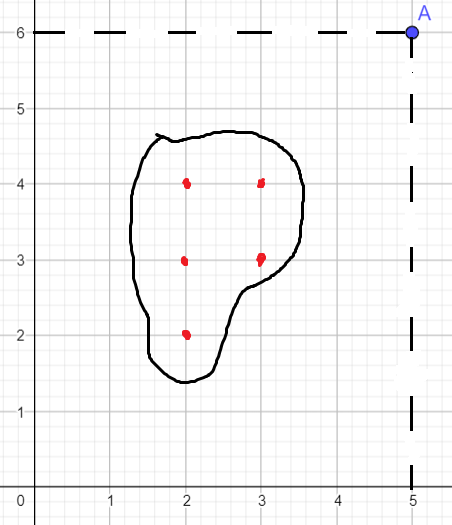
\includegraphics[width=0.39\textwidth]{image/Bai8.png}
    \vspace*{-4cm}
\end{wrapfigure}

\textbf{Ví dụ:} xét điểm $A(5, 6)$ và vũng nước như hình bên.

Ta nhận thấy rằng các điểm trên hệ trục toạ độ bị ``chìm'' trong vũng nước là\\ $\left\{(2, 2), (2, 3), (2, 4), (3, 3), (3, 4)\right\}$.\\ Vậy, $\s = \left\{(2, 2), (3, 2), (4, 2), (3, 3), (4, 3)\right\}$ (do ký hiệu toạ độ trong hệ trục $Oxy$ và ma trận bị ngược nhau).\par Khi thực hiện thuật toán, các ô mang toạ độ này sẽ chứa giá trị $0$. \par 
Vậy ta có thể thành lập một ma trận $7\times 6$ như sau (ở trang sau).\\
\pagebreak

\begin{figure}[H]
    \newcommand{\0}{\textcolor{red}{0}}
    \centering
    \begin{tikzpicture}
        \matrix[matrix of nodes,nodes={draw=gray, anchor=center, minimum size=1cm}, column sep=-\pgflinewidth, row sep=-\pgflinewidth] (A) {
            1 & 7 & 13 & 19 & 34 & \textcolor{blue}{82}\\
            1 & 6 & 6 & 6 & 15 & 48\\
            1 & 5 & \0 & \0 & 9 & 33\\
            1 & 4 & \0 & \0 & 9 & 24\\
            1 & 3 & \0 & 4 & 9 & 15\\
            1 & 2 & 3 & 4 & 5 & 6\\
            1 & 1 & 1 & 1 & 1 & 1\\};
        \end{tikzpicture}
\end{figure}

Vậy đáp số của ví dụ này là 82.

\subsection{Câu b}
\begin{wrapfigure}{L}{0.4\textwidth}
    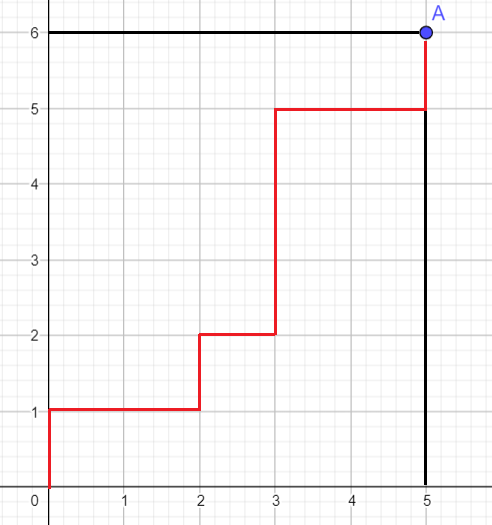
\includegraphics[width=0.39\textwidth]{image/Bai8b.png}
    \caption*{Đường đi ứng với chuỗi \cd{URRURUUURRU}}
    \vspace*{-2cm}
\end{wrapfigure}
Nếu không tồn tại vũng nước, ta nhận thấy rằng để đi từ gốc toạ độ $O$ đến $A(m, n)$ luôn luôn tốn $m+n$ bước. \par Ví dụ như xét điểm $A(5, 6)$ như hình bên, ta luôn luôn tốn $5+6=11$ bước để đi từ $O$ đến $A$.\par 
Nếu ta ký hiệu một bước đi lên là ký tự \cd U và một bước sang phải là ký tự \cd R, một đường đi sẽ tương ứng với một chuỗi các kí tự \cd{U, R}. Ta nhận thấy nếu ta đổi chỗ các kí tự \cd U hoặc các kí tự \cd R cho nhau thì chuỗi trên vẫn không thay đổi, nên bài toán sẽ trở thành: có bao nhiêu cách chọn $m+n$ kí tự từ $m$ kí tự \cd R và $n$ kí tự \cd U?\bigskip 

Số cách chọn phù hợp là:
$$
{m+n \choose m} = {m + n \choose n}
$$
\pagebreak
\section{Bài 9}
\begin{wrapfigure}{L}{0.4\textwidth}
    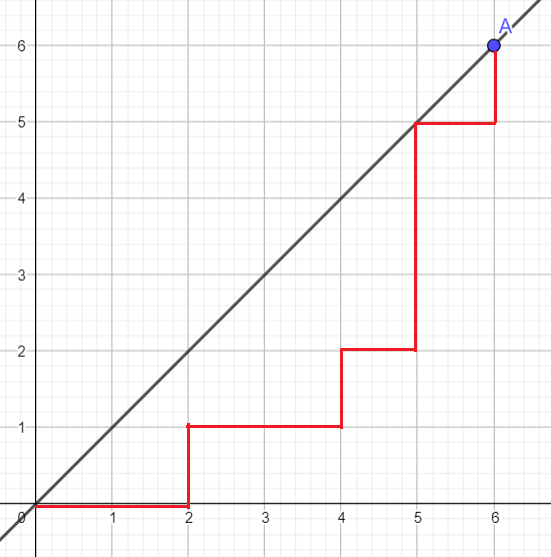
\includegraphics[width=0.39\textwidth]{image/Bai9.png}
    \vspace*{-1cm}
\end{wrapfigure}
Ta nhận thấy nếu \s là nửa mặt phẳng phía trên $OA$ không kể bờ thì ta chỉ có thể đi được các điểm nằm trên hoặc phía dưới đường thẳng $y=x$.
Khi đó, số bước đi về hướng Bắc không thể nhiều hơn số bước đi về hướng Đông. Dựa vào kết quả trong slide bài giảng, ta có thể dễ dàng nhận ra số bước đi chính là số Catalan thứ $n$:
$$
C_n = \frac{1}{n+1}{2n\choose n}
$$

\end{document}